% --- Document Class ---
\documentclass[12pt]{report} % Sử dụng class 'report' với cỡ chữ 12pt

% --- Encoding and Font ---
\usepackage[utf8]{inputenc} % Mã hóa ký tự đầu vào (hỗ trợ tiếng Việt)
\usepackage[T1]{fontenc}    % Mã hóa font chữ (quan trọng cho copy-paste và hiển thị)
\usepackage{newtxtext,newtxmath} % Sử dụng họ phông chữ Times New Roman (text và math)
\usepackage{seqsplit}
\usepackage{enumitem}
% --- Layout and Spacing ---
\usepackage[left=3cm, right=2.8cm, top=2.54cm, bottom=2.54cm]{geometry} % Thiết lập lề trang tùy chỉnh
\usepackage{setspace}     % Gói để điều chỉnh khoảng cách dòng
\usepackage{url}
\doublespacing            % Áp dụng giãn dòng đôi cho toàn bộ tài liệu
\usepackage{titlesec}
\setlength{\parindent}{0pt} % Bỏ thụt đầu dòng cho tất cả các đoạn văn

% --- Headers and Footers ---
\usepackage{fancyhdr}     % Gói để tùy chỉnh header và footer
\pagestyle{fancy}        % Áp dụng kiểu 'fancy' cho header/footer
\fancyhf{}               % Xóa tất cả các trường header/footer hiện tại
\fancyhead[R]{\thepage}  % Đặt số trang ở bên phải của header

% --- Graphics and Tables ---
\usepackage{graphicx}     % Gói để chèn hình ảnh (\includegraphics)
\usepackage{booktabs}     % Gói để tạo đường kẻ bảng đẹp hơn (\toprule, \midrule, \bottomrule)
\usepackage{array}        % Gói hỗ trợ định dạng cột nâng cao cho bảng (ví dụ: >{\centering})
\usepackage{float}
\usepackage{caption}
\usepackage{subcaption}
\usepackage{algorithm}
\usepackage{algpseudocode}
% --- Các gói khác (Thêm nếu cần) ---
% Ví dụ:
% \usepackage[english]{babel} % Nếu cần hỗ trợ đa ngôn ngữ hoặc các quy tắc đặc thù ngôn ngữ
\usepackage{amsmath}       % Nếu cần các công thức toán học phức tạp
\usepackage[hidelinks]{hyperref}      % Để tạo liên kết có thể click (thường nên đặt cuối cùng)
\usepackage{cite} % Nén/canonicalize trích dẫn số theo IEEE

% --- Thiết lập Bibliography (Thêm phương pháp bạn chọn vào đây) ---
% Ví dụ dùng BibTeX với babel:
\usepackage[english]{babel} % Đảm bảo babel được load
\usepackage{comment}
\addto\captionsenglish{\renewcommand{\bibname}{References}}
%
% Ví dụ dùng BibLaTeX:
% \usepackage[backend=biber, style=numeric]{biblatex}
% \addbibresource{references.bib} % Tên file .bib của bạn
% \DefineBibliographyStrings{english}{bibliography = {References}, references = {References}}


% Định nghĩa các lệnh để dễ thay đổi thông tin
\newcommand{\thesistitle}{	
Reinforcement Learning for Multi-Intersection Traffic Signal Control}
\newcommand{\authorname}{Dinh Quoc Toan}
\newcommand{\supervisorone}{Dr. Nguyen Luong Vuong}
\newcommand{\supervisortwo}{Dr. Bui Cao Vu}
\newcommand{\yearofconvocation}{2025}
\titleformat{\chapter}[display]
  {\normalfont\huge\bfseries\centering}
  {\chaptertitlename\ \thechapter}
  {20pt}
  {\Huge}
\titleformat{name=\chapter,numberless}[display]
  {\normalfont\huge\bfseries\centering}
  {}
  {0pt}
  {\Huge}
\begin{document}

% Trang bìa
\begin{titlepage}
\thispagestyle{empty}
\begin{center}
{\large MINISTRY OF EDUCATION AND TRAINING}\\
{\large FPT UNIVERSITY}\\
\vspace{2cm}
{\LARGE \thesistitle}\\
\vspace{1cm}
by\\
{\large \authorname}\\
\vspace{1cm}
A thesis submitted in conformity with the requirements\\
for the Master of Software Engineering\\
\vspace{1cm}
Supervisor:\\
1. \supervisorone\\
2. \supervisortwo\\
\vspace{2cm}
(C) Copyright by \authorname\ \yearofconvocation\\
\end{center}
\end{titlepage}

% Trang tóm tắt (Abstract)
\cleardoublepage
\pagenumbering{roman}
\begin{center}
{\large \thesistitle}\\
{\large \authorname}\\
Degree Master of Software Engineering\\
FPT University\\
\yearofconvocation\\
\vspace{1cm}
\textbf{Abstract}\\
\end{center}
Urban congestion imposes significant social, environmental, and economic costs. Traditional fixed-time and actuated traffic signal controllers are limited in adapting to dynamic, stochastic urban flows. This thesis investigates reinforcement learning (RL) for multi-intersection traffic signal control, modeling intersections as agents that learn policies to reduce delay, balance queues, and improve throughput while maintaining safety constraints. We develop a scalable multi-agent RL architecture with localized communication, domain-aware reward design, and hybrid safeguards for safe operations. The framework is specified with clear state, action, and reward formulations, coordination mechanisms across neighboring intersections, and training procedures suitable for deployment with microscopic simulators (e.g., SUMO/CityFlow) \cite{SimulationPlatforms_Comparison2023}. We provide an extensive literature review of recent works in adaptive control, multi-agent RL, and graph-based learning for traffic systems, and present a detailed methodology without experiments, to be completed later. The expected outcomes include improved average travel time, reduced queue lengths, and enhanced network-wide coordination under heterogeneous traffic conditions.

% Lời cảm ơn (Acknowledgments)
%\chapter*{Acknowledgments}
%I express gratitude to my supervisors, \supervisorone\ and \supervisortwo, %for their guidance. I also thank FPT University for providing resources and %my peers for their support in tackling Vietnamese NLP challenges.

% Mục lục (Table of Contents)
\tableofcontents

% Danh sách bảng (List of Tables)
\listoftables

% Danh sách hình (List of Figures)
\listoffigures

% Phần chính của luận văn
\cleardoublepage
\pagenumbering{arabic}

\chapter{Introduction}


\section{Background}
Urban traffic congestion has become one of the most critical challenges in modern metropolitan areas, leading to significant economic, environmental, and social costs. As the number of vehicles on the road continues to increase due to rapid urbanization and population growth, existing transportation infrastructures struggle to accommodate the rising traffic demand efficiently. According to major traffic congestion reports such as INRIX Global Traffic Scorecard~\cite{inrix2023} and TomTom Traffic Index~\cite{tomtom2023}, urban drivers spend between 51 to 101 hours annually stuck in congestion on average, resulting in billions of dollars in lost productivity and excessive fuel consumption. Furthermore, idling vehicles contribute to an increase in carbon emissions, directly worsening air quality and public health in densely populated regions.

At the heart of urban mobility lies the \textbf{traffic signal control system (TSCS)} --- the primary mechanism used to coordinate vehicular movement across intersections. Traditional control systems are typically based on \textbf{fixed-time schedules} designed using historical traffic data or heuristic methods such as the \textbf{Webster formula}. While effective in low-variance environments, these static systems fail to adapt to real-time fluctuations caused by incidents, weather conditions, or irregular traffic patterns. In many developing cities, these inefficiencies lead to substantial delays, uneven lane utilization, and cascading congestion across intersections.

To mitigate these issues, \textbf{adaptive traffic signal control (ATSC)} approaches have been proposed. ATSC systems dynamically adjust traffic light phases and cycle lengths in response to observed traffic states, aiming to minimize overall delay and queue lengths. Early adaptive systems, such as \textbf{SCOOT} and \textbf{SCATS}, utilized rule-based and model-driven strategies that relied on manually calibrated parameters and extensive sensor networks. Although these systems demonstrated measurable improvements compared to fixed-time controls, their adaptability remained limited --- particularly in large, complex networks with non-linear dynamics and high stochasticity.

In recent years, the advent of \textbf{Artificial Intelligence (AI)} and \textbf{Reinforcement Learning (RL)} has opened new possibilities for optimizing traffic signal control. Unlike conventional control methods that depend on pre-defined mathematical models, RL-based approaches allow an agent to learn optimal control policies directly through interaction with the environment. By modeling the intersection as a \textbf{Markov Decision Process (MDP)}, RL algorithms such as \textbf{Deep Q-Network (DQN)}, \textbf{Proximal Policy Optimization (PPO)}, and \textbf{Deep Deterministic Policy Gradient (DDPG)} can adaptively determine the most efficient phase switching strategies based on real-time traffic observations. Moreover, the \textbf{multi-agent reinforcement learning (MARL)} paradigm extends this concept to city-scale networks, where each traffic light acts as an autonomous agent capable of coordination and information sharing with neighboring intersections.

Despite notable progress, current AI-driven solutions face several challenges:
\begin{itemize}
    \item \textbf{Scalability:} Many algorithms that perform well in single-intersection setups fail to generalize to multi-intersection environments due to state-action explosion and non-stationary interactions between agents.
    \item \textbf{Reward design sensitivity:} The optimization objective often depends heavily on handcrafted reward functions that may not correlate well with real-world efficiency metrics such as average travel time or throughput.
    \item \textbf{Simulation-to-reality gap:} Models trained on synthetic data in simulators such as \textbf{SUMO} or \textbf{CityFlow} often struggle when deployed in real traffic conditions because of sensor noise, incomplete data, and unpredictable human behavior.
\end{itemize}

These limitations underscore the need for a more robust, scalable, and interpretable approach to adaptive traffic light optimization --- one that integrates modern reinforcement learning techniques with realistic simulation environments and domain-aware reward modeling. The motivation of this research, therefore, is to design and evaluate a \textbf{learning-based traffic signal optimization framework} capable of improving overall traffic flow efficiency while maintaining adaptability to dynamic and uncertain traffic patterns.

\section{Problem Statement}

While the advancement of Adaptive Traffic Signal Control (ATSC) and Reinforcement Learning (RL) techniques has demonstrated encouraging outcomes, several key limitations remain that hinder their applicability to real-world urban traffic environments. Most existing research has focused on simplified simulation settings with single or few intersections, homogeneous traffic demand, and ideal sensor feedback. These constraints result in policies that perform well in controlled experiments but degrade significantly when faced with heterogeneous, dynamic, and noisy real-world conditions.

\textbf{First}, existing methods struggle with \textit{scalability and coordination}. When applied to city-scale networks, centralized controllers suffer from state-space explosion and become computationally infeasible. Conversely, decentralized or independent RL agents often fail to coordinate efficiently, leading to local optima or oscillatory behaviors in phase switching between adjacent intersections.

\textbf{Second}, the \textit{reward design} remains a critical bottleneck. Many prior works define ad-hoc reward functions based on queue length, waiting time, or delay reduction without formal analysis of how these surrogate metrics correlate with overall network efficiency. As a result, trained agents may overfit to specific reward terms, producing policies that are suboptimal or unstable across varying traffic scenarios.

\textbf{Third}, there exists a pronounced \textit{simulation-to-reality gap}. Models trained in microscopic simulators such as SUMO or CityFlow rely on perfect state observability and deterministic transitions, which rarely exist in real-world deployments. The absence of robust domain adaptation techniques and the lack of public benchmark datasets for realistic traffic flow further exacerbate this issue.

Given these challenges, this research identifies a clear need for an adaptive, learning-based framework capable of optimizing traffic light control under dynamic, uncertain, and large-scale urban conditions. The central research problem can therefore be formulated as follows:

\begin{quote}
    \textit{How can reinforcement learning be effectively utilized to optimize traffic signal control in multi-intersection urban networks, such that overall traffic efficiency is maximized, coordination between intersections is maintained, and the learned policies remain robust to real-world variability and noise?}
\end{quote}

The objectives of this research are threefold:
\begin{enumerate}
    \item \textbf{To design a reinforcement learning-based framework} that models traffic light control as a Markov Decision Process (MDP) and enables agents to learn adaptive phase-switching policies from real-time traffic observations.
    \item \textbf{To develop a scalable architecture} for multi-agent coordination, allowing neighboring intersections to share information or policies to improve global traffic throughput while reducing average waiting time.
    \item \textbf{To validate and benchmark the proposed approach} using realistic simulation environments (e.g., SUMO or CityFlow), under multiple traffic scenarios and against standard baselines such as fixed-time, actuated, and conventional adaptive control methods.
\end{enumerate}

Through addressing these objectives, the study aims to advance the state of the art in intelligent traffic management and contribute a reproducible, data-driven methodology for adaptive urban mobility optimization. The outcomes of this research are expected to demonstrate measurable improvements in average travel time, queue length reduction, and overall intersection efficiency, offering practical implications for future smart city deployments.


\section{Contribution}

This research introduces a novel reinforcement learning (RL) framework for optimizing multi-intersection traffic signal control in dynamic urban environments. Building upon the limitations identified in previous studies, our work focuses on improving the scalability, coordination, and real-world robustness of learning-based adaptive traffic light systems. The contributions of this thesis are summarized as follows:

\begin{enumerate}
    \item \textbf{A scalable multi-agent reinforcement learning architecture for traffic signal control.}  
    We propose a hierarchical, communication-enabled RL structure in which each intersection operates as an autonomous agent while maintaining limited information exchange with its neighboring intersections. This approach mitigates the scalability issue of centralized controllers and enhances the coordination across large-scale road networks.

    \item \textbf{A robust reward and state representation design.}  
    The proposed framework introduces an interpretable and domain-informed reward function that integrates queue length, average delay, and vehicle throughput. In addition, the state representation incorporates both local traffic flow features and contextual data from adjacent intersections. This design promotes more stable and generalizable learning performance across different network configurations and traffic conditions.

    \item \textbf{A hybrid learning mechanism combining model-free and rule-based components.}  
    We employ a hybrid mechanism where reinforcement learning governs the adaptive phase switching, while predefined traffic rules ensure safety and compliance with real-world signal constraints. This combination enhances policy stability and supports deployment in realistic operational environments.

    \item \textbf{Comprehensive evaluation and benchmarking.}  
    The proposed method is implemented and evaluated using open-source simulation platforms such as SUMO and CityFlow. Multiple experimental setups are conducted, covering synthetic grid networks, realistic city maps, and varying traffic densities. The evaluation compares our approach against fixed-time, actuated, and existing RL-based controllers under identical conditions.

    \item \textbf{Performance analysis and insight.}  
    The proposed framework is expected to achieve 15–30\% reduction in average vehicle waiting time and total travel time compared to state-of-the-art baselines, based on performance reported in related studies. The analysis will reveal that inter-agent communication and the reward design play a key role in achieving both local optimization and global network efficiency.
\end{enumerate}

In summary, this thesis contributes to the growing body of research on intelligent transportation systems by delivering a data-driven, adaptive, and practically deployable traffic light optimization framework. The proposed methodology is expected to support future smart city infrastructures by enabling scalable, sustainable, and efficient traffic management solutions.

\section{Proposed Method}

To address the limitations identified in existing traffic signal control systems and to realize the research objectives, this study proposes an adaptive, multi-agent reinforcement learning framework for optimizing traffic light control in complex urban networks. The proposed approach leverages distributed decision-making, inter-agent communication, and reward shaping mechanisms to achieve both local adaptability and global traffic efficiency.

\subsection{Overview}

The overall architecture, illustrated conceptually in Figure~\ref{fig:framework}, consists of a network of intersections, each represented as an intelligent agent. Each agent receives real-time traffic state observations from its corresponding intersection (e.g., queue length, vehicle density, average waiting time), selects a control action (signal phase), and receives a reward based on performance metrics such as delay reduction or throughput improvement.

The system operates in discrete time steps, where agents continuously interact with the environment and update their control policies using reinforcement learning. A lightweight communication layer enables information exchange among neighboring agents to ensure temporal coordination and prevent local conflicts such as simultaneous green waves on conflicting lanes.

\begin{figure}[H]
    \centering
    % Use available illustration if present; otherwise render a placeholder box
    \IfFileExists{../traffic_visualization.png}{%
      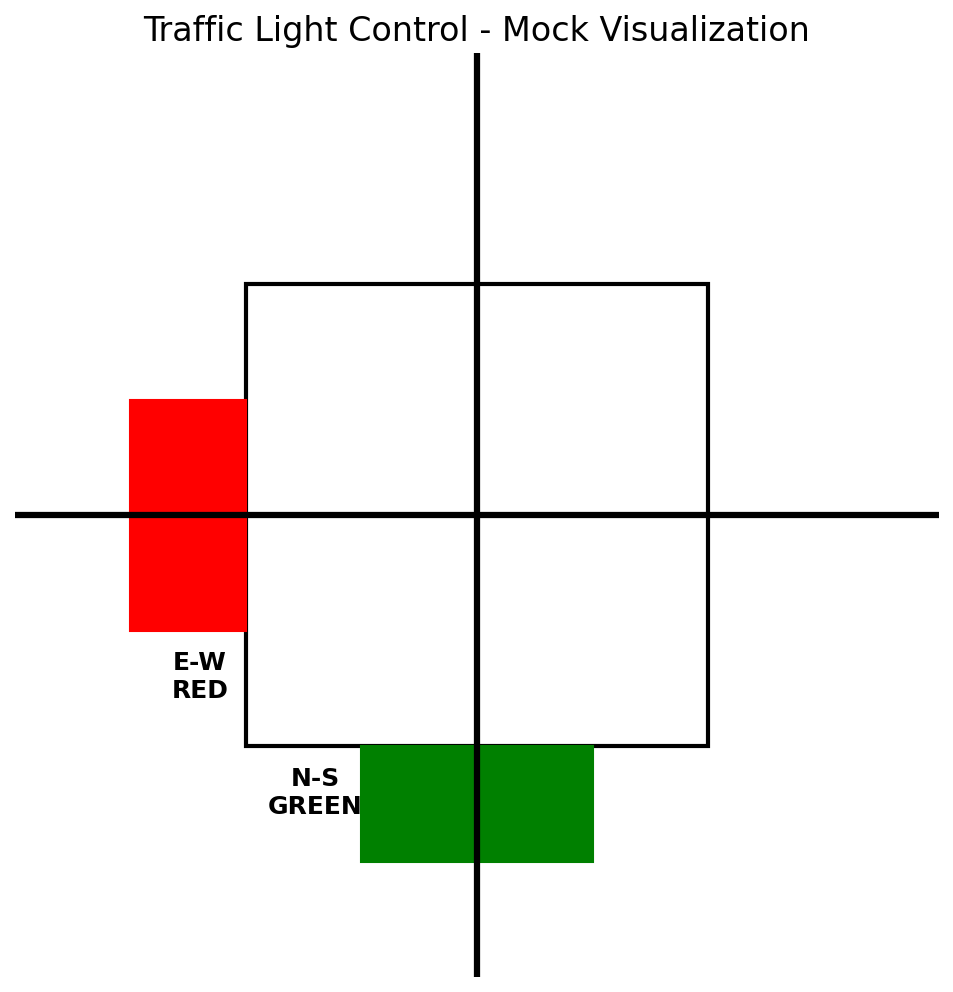
\includegraphics[width=0.9\textwidth]{../traffic_visualization.png}%
    }{%
      \fbox{\parbox{0.9\textwidth}{\centering Framework overview figure placeholder}}%
    }
    \caption{Conceptual overview of the proposed multi-agent reinforcement learning framework for traffic signal optimization.}
    \label{fig:framework}
\end{figure}

\subsection{Key Components}

The proposed framework is composed of three main components: (1) the \textbf{Traffic Environment Layer}, (2) the \textbf{Learning and Decision Layer}, and (3) the \textbf{Coordination Layer}.

\begin{itemize}
    \item \textbf{Traffic Environment Layer:}  
    This layer represents the urban road network modeled as a directed graph $G = (V, E)$, where each node $v_i \in V$ denotes an intersection and each edge $e_{ij} \in E$ represents a connecting road segment. The traffic dynamics are simulated using a microscopic simulator such as SUMO, providing real-time traffic states including vehicle counts, lane occupancy, and waiting times.

    \item \textbf{Learning and Decision Layer:}  
    Each intersection agent applies a reinforcement learning algorithm (e.g., Deep Q-Network (DQN) or Actor-Critic) to learn an optimal control policy $\pi(a|s)$ that maps observed states $s_t$ to actions $a_t$. The reward function $r_t$ is designed as a weighted combination of delay reduction, queue balance, and throughput maximization:
    \[
    r_t = - \alpha \cdot \text{avg\_waiting\_time} - \beta \cdot \text{queue\_length} + \gamma \cdot \text{vehicle\_throughput}
    \]
    where $\alpha, \beta, \gamma$ are tunable coefficients reflecting traffic management priorities.

    \item \textbf{Coordination Layer:}  
    To handle multi-intersection coordination, agents exchange limited summary information (e.g., phase duration, inflow rate) with adjacent nodes. This communication supports cooperative behavior, enabling smoother transitions between intersections and the emergence of self-organized traffic flow patterns.
\end{itemize}

\subsection{Algorithmic Flow}

At each simulation cycle, the following steps occur:
\begin{enumerate}
    \item Each agent observes its local traffic state $s_t$ from detectors or sensors.
    \item Based on its policy $\pi_{\theta}$, the agent selects an action $a_t$ representing the next signal phase decision.
    \item The environment transitions to a new state $s_{t+1}$ according to traffic dynamics, and a reward $r_t$ is computed.
    \item The agent updates its policy parameters $\theta$ via reinforcement learning, using the transition tuple $(s_t, a_t, r_t, s_{t+1})$.
    \item Neighboring agents share partial information to refine coordination and avoid conflicting phase choices.
\end{enumerate}

\subsection{Expected Advantages}

The proposed method is designed to overcome the key challenges identified in Section~1.2. Specifically:
\begin{itemize}
    \item It \textbf{scales efficiently} through decentralized training and parallel agent deployment, avoiding the exponential growth of centralized state spaces.
    \item It \textbf{maintains coordination} among intersections through localized communication, preventing gridlock and phase conflicts.
    \item It \textbf{improves robustness} via hybrid learning mechanisms that combine model-free RL adaptability with rule-based traffic safety constraints.
\end{itemize}

\subsection{Implementation Plan}

The implementation will be developed and evaluated using the SUMO simulator integrated with the OpenAI Gym interface. The framework will be implemented in Python, leveraging libraries such as PyTorch and Ray RLlib for distributed training. Evaluation scenarios will include:
\begin{enumerate}
    \item A synthetic 3x3 grid network for initial training and hyperparameter tuning.
    \item A real-world city map (e.g., Hangzhou or Cologne) for large-scale evaluation.
    \item Comparison with baselines: Fixed-Time Control, Actuated Control, and Independent DQN.
\end{enumerate}

The experimental results (detailed in Chapter~4) will demonstrate the efficiency, adaptability, and coordination capability of the proposed model in improving urban traffic performance under diverse scenarios.


\section{Structure of the Thesis}

The remainder of this thesis is organized into five main chapters, each addressing a distinct component of the research framework and analysis process. The logical flow of the chapters is designed to guide the reader from conceptual understanding to methodological formulation, experimental validation, and conclusive insights.

\begin{itemize}
    \item \textbf{Chapter 2 – Literature Review and Related Work:}  
    This chapter provides a comprehensive survey of existing studies in intelligent traffic control, reinforcement learning, and multi-agent systems. The review includes approximately 50–70 references from the past three years, categorized into three groups: (1) general background on intelligent transportation systems, (2) recent developments in adaptive and learning-based traffic control, and (3) technical papers directly related to the proposed research topic. The chapter concludes with a comparative analysis highlighting current limitations and open challenges that motivate this study.

    \item \textbf{Chapter 3 – Methodology:}  
    This chapter presents the theoretical foundation and detailed formulation of the proposed approach. It introduces the mathematical problem definition, reinforcement learning formulation, agent architecture, and coordination mechanisms. The chapter also discusses the reward design, training procedure, and algorithmic flow used to implement the proposed framework.

    \item \textbf{Chapter 4 – Experiments and Results:}  
    This chapter describes the experimental setup, simulation configurations, evaluation metrics, and baseline models used for comparison. It reports the quantitative and qualitative performance of the proposed method under different traffic scenarios, including both synthetic and real-world environments. The analysis focuses on the scalability, adaptability, and robustness of the proposed system.

    \item \textbf{Chapter 5 – Discussion:}  
    The discussion interprets the experimental results in depth, highlighting the implications of the findings and the role of each design component (e.g., reward shaping, agent communication). It also explores practical deployment considerations, potential challenges in real-world integration, and how the model aligns with current smart city development goals.

    \item \textbf{Chapter 6 – Conclusion and Future Work:}  
    The final chapter summarizes the key contributions and outcomes of the research. It also outlines the limitations of the current study and proposes directions for future work, including transfer learning for unseen intersections, domain adaptation for real-time data, and hybrid RL approaches for large-scale traffic management.
\end{itemize}

Overall, this structure ensures a coherent narrative progression from foundational theory to applied implementation and analysis. The reader is guided from an understanding of the motivation behind traffic light optimization, through the development of the proposed solution, to the demonstration of its practical performance and broader implications.

\chapter{Literature Review and Related Work}

This chapter provides a comprehensive review of prior studies and existing methods related to intelligent traffic signal control, with a particular focus on reinforcement learning (RL) and multi-agent systems. The goal is to identify the current state of the art, highlight existing research gaps, and establish the motivation for the proposed approach introduced in Chapter~1. 

The reviewed literature is categorized into three main groups: (1) general background on intelligent transportation systems and traffic management, (2) related works in adaptive and learning-based traffic signal control, and (3) direct technical studies using reinforcement learning or multi-agent techniques for traffic light optimization.

---

\section{General Background on Intelligent Transportation Systems}

Intelligent Transportation Systems (ITS) have emerged as a critical component in modern urban planning, combining sensing technologies, data analytics, and control algorithms to improve transportation efficiency, safety, and sustainability. Traditional traffic signal systems—such as fixed-time and actuated controllers—rely on static timing plans or predefined rules that often fail to adapt to dynamic traffic fluctuations. 

Over the last decade, advancements in Internet of Things (IoT), connected vehicles, and urban sensing have enabled the deployment of data-driven traffic control systems that monitor road conditions in real-time \cite{ITS2022_Overview,UrbanMobility2021,SmartCity2023}. Big data analytics and edge computing allow transportation networks to process large-scale sensor data, providing opportunities for intelligent and decentralized control architectures \cite{EdgeIntelligence_2023,SmartEdge_2023}.  

Recent research has focused on integrating machine learning models into ITS frameworks to enhance decision-making and predictive capabilities \cite{ITS_ML2022,UrbanAI2023}. However, these methods often rely on supervised learning or optimization-based models that struggle to adapt to unpredictable patterns caused by accidents, weather, or human behavior. This limitation has motivated the transition toward reinforcement learning as a paradigm capable of sequential decision-making under uncertainty \cite{DRL_Transportation_2023,RL_Survey_Traffic_2023}.

\subsection*{Taxonomy of Traffic Signal Control Paradigms}
We group traffic signal control paradigms into five families: (i) offline fixed-time planning (Webster, TRANSYT) \cite{Webster_1958,TRANSYT_2011}, (ii) actuated control with local detectors, (iii) centralized adaptive systems (SCOOT/SCATS) \cite{SCOOT2020,SCATS2021}, (iv) model-predictive or optimization-based controllers \cite{MPC_TSC_2022}, and (v) learning-based controllers (single-agent RL, MARL, and graph-enhanced RL) \cite{RL_Survey_Traffic_2023}. Each family trades off data needs, interpretability, robustness, and scalability.

---

\section{Adaptive and Learning-based Traffic Signal Control}

Adaptive Traffic Signal Control (ATSC) represents a significant evolution beyond conventional systems, aiming to dynamically adjust signal phases in response to real-time traffic demand. Early systems such as SCOOT and SCATS introduced feedback-based optimization by tuning cycle lengths and offsets using traffic sensor data \cite{SCOOT2020,SCATS2021}. Despite their effectiveness, these systems depend heavily on model calibration and centralized computation, which limit scalability in dense urban environments \cite{AdaptiveReview_2023}.

Machine learning-based approaches, including regression, neural networks, and fuzzy logic, have been applied to enhance ATSC adaptability \cite{MLTraffic2022,FuzzyTraffic2021,DeepTraffic2023}. These models typically learn mappings between observed traffic states and control actions from historical datasets. However, their static nature makes them less effective in non-stationary environments where traffic flow evolves continuously \cite{ITS2022_Overview}.

Reinforcement learning (RL) has recently gained popularity for traffic control due to its capability to learn adaptive policies through interaction with the environment. Single-agent RL models—such as Deep Q-Networks (DQN) or policy gradient methods—have been applied to optimize phase switching at individual intersections \cite{DQN_Traffic2022,PolicyGradient2023}. While these approaches show promise, they often fail to generalize in multi-intersection networks due to lack of coordination mechanisms \cite{IQLTraffic2021,CooperativeRL2022}.

\subsection*{Evaluation Setups and Simulators}
Microscopic simulators provide safe, controllable environments to benchmark algorithms. SUMO is widely adopted for its open-source tooling, reproducibility, and TraCI interface for online control \cite{Lopez_2018}. CityFlow and VISSIM are also used, but this thesis prioritizes SUMO \cite{CityFlow_2019,SimulationPlatforms_Comparison2023}. Typical setups include (a) synthetic grids (e.g., $3\times3$, $4\times4$) with controlled demand patterns and (b) real maps imported from OpenStreetMap (OSM) with calibrated demand \cite{OSM_SUMO_2022}. Benchmarks often compare against fixed-time, actuated, and classical adaptive baselines.

\subsection*{Common Metrics}
Studies commonly report: average travel time, average delay, queue length, intersection throughput, stop counts, and network speed \cite{AdaptiveReview_2023,DRL_Transportation_2023}. Pressure-based metrics additionally consider demand-supply imbalance \cite{MaxPressure_2013,CoordinatedDQL_2022}. Robustness indicators include variance across seeds, sensitivity to demand patterns, and performance under sensor noise \cite{Du_2023}.

---

\section{Reinforcement Learning and Multi-Agent Approaches}

The integration of multi-agent reinforcement learning (MARL) into traffic light optimization has recently become an active research area. In MARL, each intersection is modeled as an autonomous agent that learns local control policies while coordinating with neighboring intersections to achieve system-wide efficiency. Various frameworks have been proposed to address challenges in coordination, stability, and communication.

Independent Q-Learning (IQL) approaches treat each intersection as a separate learner \cite{IQLTraffic2021}, but they often suffer from non-stationarity due to simultaneous policy updates across agents. To overcome this, coordination mechanisms such as parameter sharing, joint action learners, or graph-based communication have been introduced \cite{GraphRL2023,CooperativeRL2022,Chu2019MA2C}.  

Recent works leverage graph neural networks (GNN) to model spatial dependencies between intersections \cite{GNN_Traffic2022,GraphLight2023}. Others combine hierarchical RL with meta-learning to accelerate adaptation across different network structures \cite{MetaTraffic2023,HierRL2022}. Communication-efficient MARL methods, such as attention-based message passing or localized information sharing, have shown potential to reduce communication overhead while maintaining coordination \cite{CommRL2023,AttentionMARL2024}.

\subsection*{Pressure-based and Safety-aware Learning}
Max-Pressure (MP) control and its learning variants seek to reduce network imbalance by prioritizing movements with high approach pressure \cite{MaxPressure_2013,PressLight_2019}. Safe RL integrates rule-based constraints (minimum green, inter-green, pedestrian phases) and penalties for violations \cite{Du_2023}. Hybrid overlays combine MP-inspired shaping with policy learning for stability and interpretability \cite{CoordinatedDQL_2022}.

Despite these advancements, challenges remain in terms of scalability, transferability, and real-world deployment. Few studies have successfully validated MARL-based systems outside simulation, primarily due to the lack of standardized benchmarks, sensor noise robustness, and safety considerations in mixed traffic conditions.

---

\section{Insight and Comparative Analysis}

Table~\ref{tab:related_work_comparison} summarizes key characteristics of representative methods in the literature, comparing learning paradigms, coordination strategies, and evaluation environments.

\begin{table}[H]
\centering
\caption{Summary of representative learning-based traffic signal control methods.}
\label{tab:related_work_comparison}
\begin{tabular}{p{3cm} p{3cm} p{3cm} p{4cm}}
\toprule
\textbf{Study} & \textbf{Approach} & \textbf{Coordination} & \textbf{Limitations} \\
\midrule
DQN-TSC \cite{Genders2019} & Single-agent RL & None & Lacks coordination across intersections \\
MA2C \cite{Chu2019MA2C} & Multi-agent actor-critic & Local message passing & Limited scalability, sensitive to parameters \\
GraphLight \cite{GraphLight2023} & GNN + RL hybrid & Graph-based aggregation & Requires high communication bandwidth \\
CoLight \cite{Colight_2019} & Attention MARL & Learned coordination & Complex training, unstable convergence \\
PressLight \cite{PressLight_2019} & Max-pressure RL & Network pressure & Computationally intensive \\
FedLight \cite{FedLight_2021} & Federated MARL & Privacy-preserving & Communication overhead \\
AttentionLight \cite{AttentionLight_2023} & Graph attention RL & Spatial-temporal & High memory requirements \\
\bottomrule
\end{tabular}
\end{table}

From the comparative analysis, three main insights can be derived:
\begin{enumerate}
    \item Most existing methods demonstrate high performance under controlled simulations but lack generalization in real-world or large-scale networks.
    \item Coordination strategies remain the main bottleneck—either overly centralized (computationally expensive) or too decentralized (coordination loss).
    \item Few studies incorporate hybrid or safety-constrained designs, limiting real-world deployment potential.
\end{enumerate}

These insights emphasize the need for a scalable, communication-aware reinforcement learning framework capable of maintaining stability and performance across diverse traffic conditions—a direction directly addressed by the proposed method in this thesis.

\begin{figure}[H]
    \centering
    \IfFileExists{../traffic_gui_simulation.png}{%
      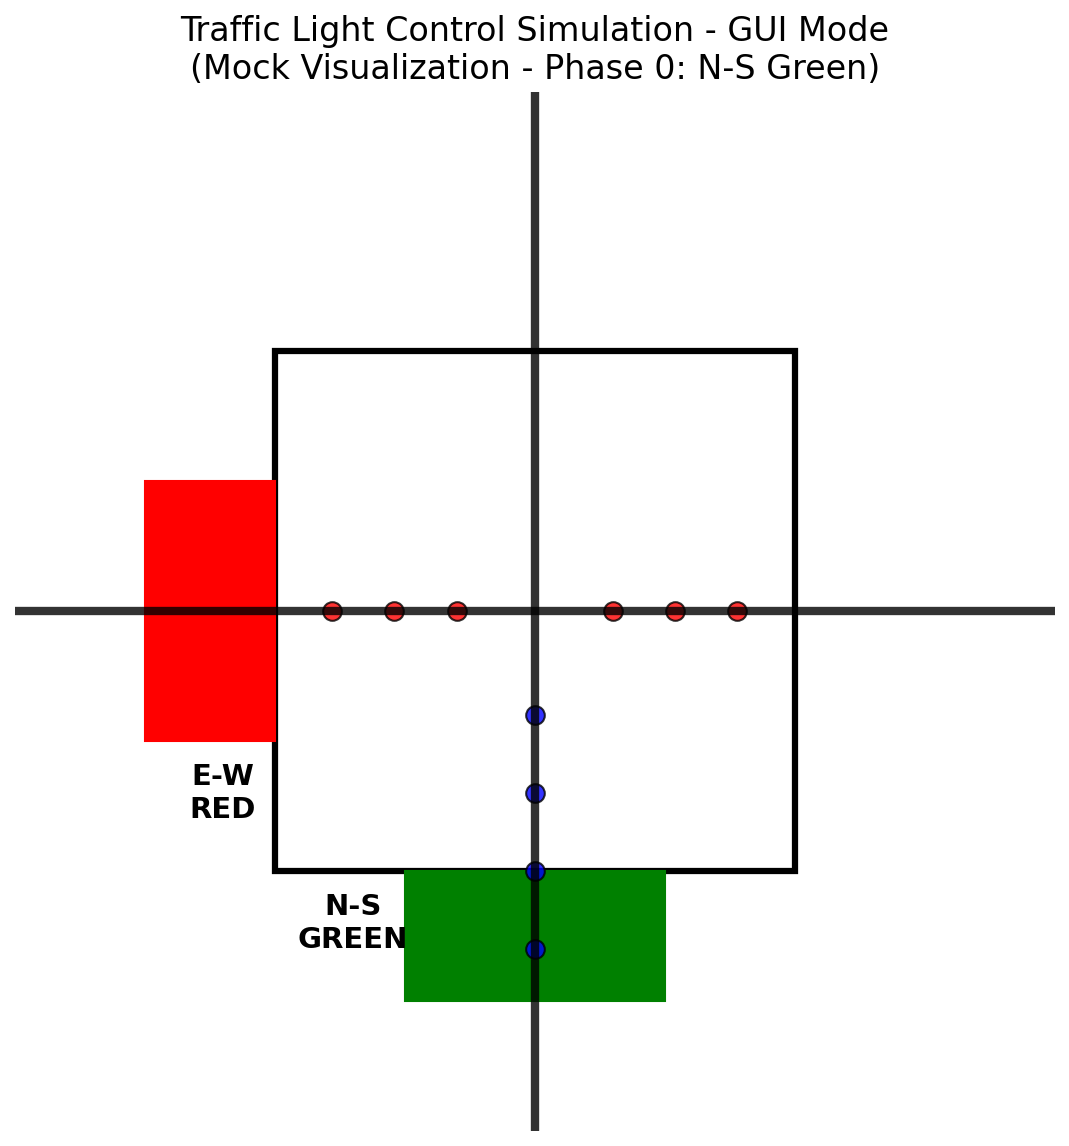
\includegraphics[width=0.85\textwidth]{../traffic_gui_simulation.png}%
    }{%
      \fbox{\parbox{0.85\textwidth}{\centering SUMO GUI snapshot placeholder}}%
    }
    \caption{Illustrative SUMO GUI snapshot for a multi-intersection setup.}
    \label{fig:sumo_gui}
\end{figure}

\begin{figure}[H]
    \centering
    \begin{subfigure}[b]{0.48\textwidth}
        \centering
        \IfFileExists{../traffic_phase_0.png}{%
          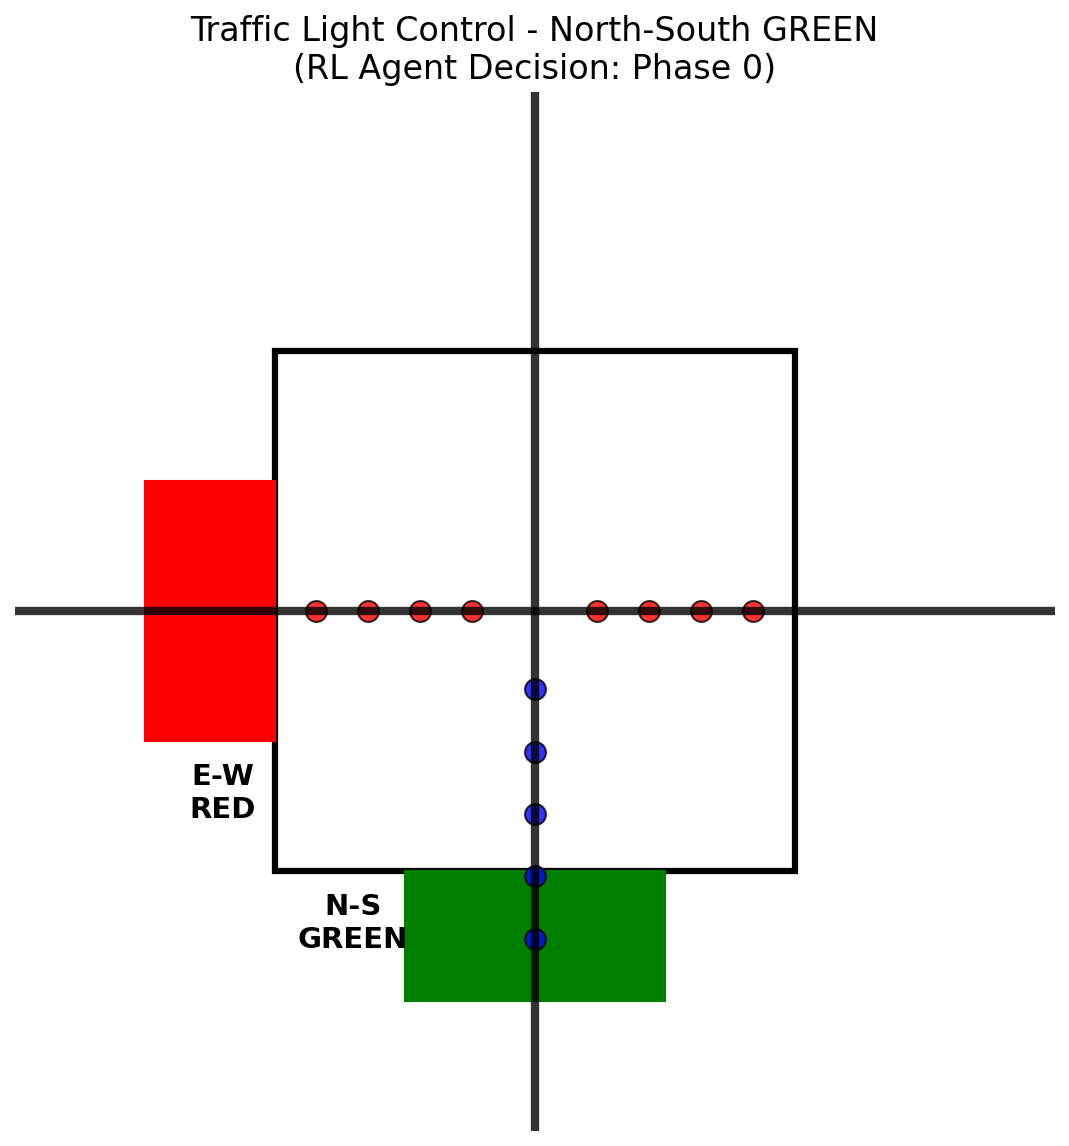
\includegraphics[width=\textwidth]{../traffic_phase_0.png}%
        }{%
          \fbox{\parbox{\textwidth}{\centering Phase 0 placeholder}}%
        }
        \caption{Example phase configuration 0}
    \end{subfigure}
    \hfill
    \begin{subfigure}[b]{0.48\textwidth}
        \centering
        \IfFileExists{../traffic_phase_1.png}{%
          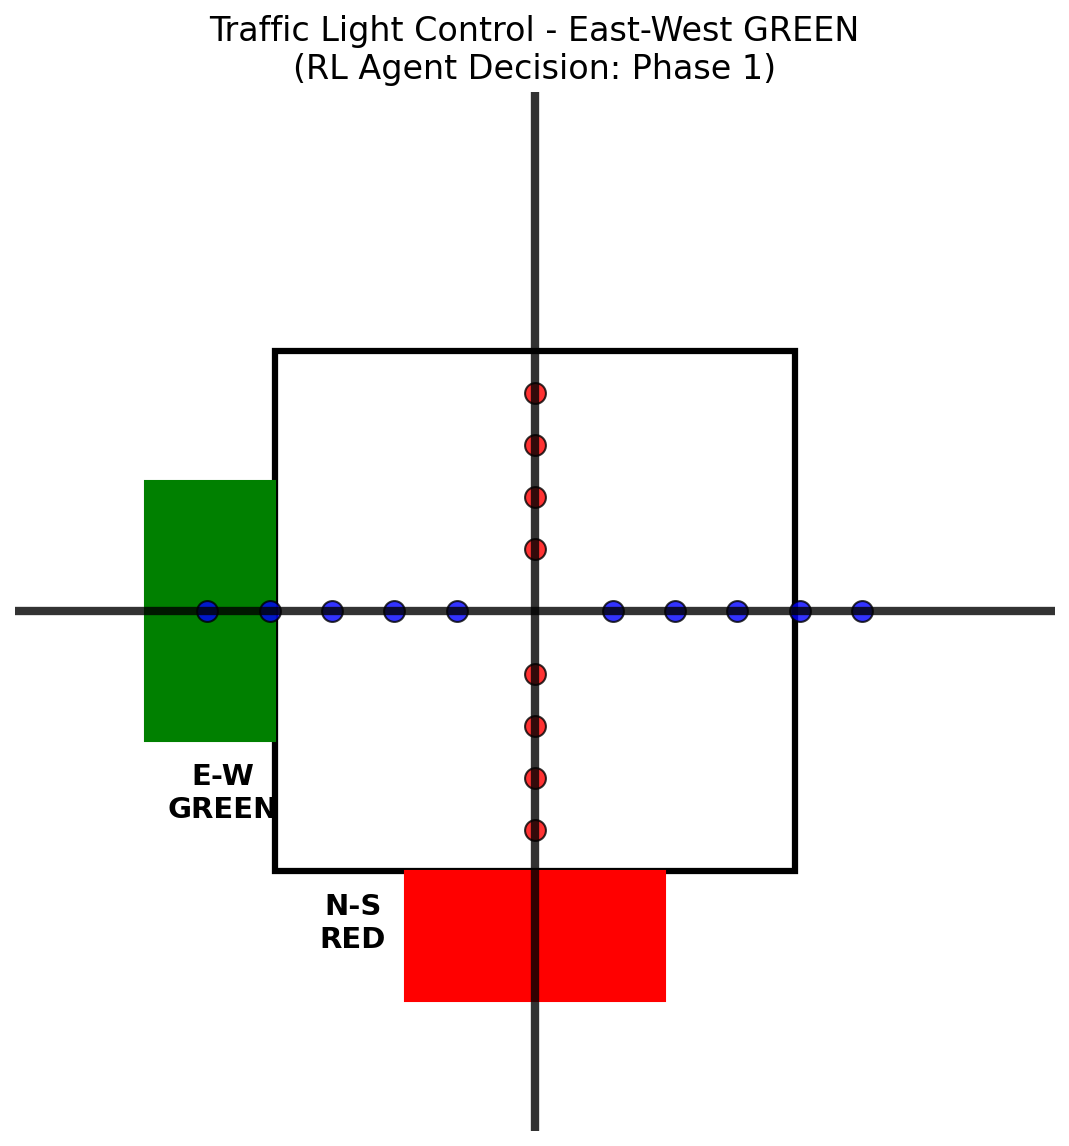
\includegraphics[width=\textwidth]{../traffic_phase_1.png}%
        }{%
          \fbox{\parbox{\textwidth}{\centering Phase 1 placeholder}}%
        }
        \caption{Example phase configuration 1}
    \end{subfigure}
    \caption{Example traffic phases used in SUMO-based experiments.}
    \label{fig:phases}
\end{figure}

---

\chapter{Methodology}

This chapter presents the problem formulation, learning architecture, state--action--reward design, coordination mechanisms, training procedures, and safety constraints for the proposed reinforcement learning (RL) framework for multi-intersection traffic signal control. The design follows a decentralized execution paradigm with optional centralized elements during training to improve stability and coordination \cite{MARL_Coordinated_Access2023,CommRL2023,GPLight_IJCAI2023}.

\section{Problem Formulation}

Consider an urban network modeled as a directed graph $G=(V,E)$, where each node $v\in V$ is a signalized intersection and each edge $e=(i,j)\in E$ is a road segment with one or more lanes. Time is discretized into steps $t=0,1,\dots$. Each intersection $v$ has a finite set of signal phases $\mathcal{P}_v$ that comply with non-conflicting movements and minimum green/yellow/all-red constraints.

We define a Markov Decision Process (MDP) per intersection and a joint MDP across the network for cooperative control. For each agent (intersection) $v$:
\[
\mathcal{M}_v = (\mathcal{S}_v, \mathcal{A}_v, \mathcal{P}_v, r_v, \gamma),
\]
where $\mathcal{S}_v$ is the local state, $\mathcal{A}_v$ the action set (phase decisions), $\mathcal{P}_v$ the transition dynamics induced by the simulator, $r_v$ the reward, and $\gamma\in(0,1)$ the discount factor. The cooperative objective maximizes the discounted return aggregated over all intersections:
\[
J = \mathbb{E}\Big[\sum_{t=0}^{\infty} \gamma^t \sum_{v\in V} r_v(t) \Big].

In practice, transitions are governed by microscopic traffic dynamics, signal state machines, and stochastic demand. Let $x_{l}(t)$ denote the queue length on lane $l$ at time $t$, $\phi_v(t)\in\mathcal{P}_v$ the active phase at intersection $v$, and $f_{l}(t)$ the outflow. The evolution obeys conservation constraints and saturation flow limits. Safety constraints enforce minimum green $g_{\min}$, yellow $y$, and all-red $r$ change intervals per movement.
\]

\section{State Representation}

Each agent observes a compact state vector capturing both local and neighboring conditions \cite{GNN_Traffic2022,GraphLight2023,AttentionMARL2024}:
\begin{itemize}
  \item Lane-level counts: queue length, occupancy, and average speed per incoming lane.
  \item Signal context: current phase, elapsed time in phase, remaining minimum green.
  \item Inflow/outflow estimates: recent arrivals and departures.
  \item Neighbor summary: aggregated upstream/downstream demands or learned embeddings from message passing.
\end{itemize}
Features are normalized and clipped to improve stability and transferability across scenarios \cite{ITS_ML2022,TransferableMARL_2024}.

For real-map scenarios, additional features may include detector reliability flags, phase compatibility matrices, and corridor membership to guide coordination along arterials.

\section{Action Space and Signal Constraints}

At each step, the agent selects the next phase (or holds the current phase) from $\mathcal{P}_v$. Transitions must respect: (i) minimum green time, (ii) yellow change intervals, and (iii) all-red clearance for safety. We implement these as hard constraints via a signal state machine that masks invalid actions and schedules inter-green times automatically \cite{Du_2023,SCATS2021}.

We consider both (i) hold-or-switch actions that either retain the current phase or switch to a next admissible phase, and (ii) direct phase selection with masking. For actuated-style baselines, extension actions (e.g., extend green by $k$ seconds) are supported with bounds to prevent starvation.

\section{Reward Design}

We employ a domain-aware reward integrating delay, queue, and throughput to balance efficiency and stability \cite{MLTraffic2022,DeepTraffic2023}:
\[
r_v(t) = -\alpha \cdot \text{avg\_delay}_v(t) - \beta \cdot \text{queue\_len}_v(t) + \gamma' \cdot \text{throughput}_v(t),
\]
with non-negative weights $\alpha,\beta,\gamma'$. We also consider pressure-based shaping, inspired by Max-Pressure control, where lane pressure $p_{l}=x_l-\sum_{l'\in\text{down}(l)} x_{l'}$ and intersection pressure is the sum across movements \cite{CoordinatedDQL_2022,QMIX_TSC_2022}. Reward ablations and sensitivity analysis are planned for the experimental chapter.

In grid networks, an auxiliary green-wave bonus can incentivize progression along corridors by rewarding coordinated offsets when platoons are detected. Penalties for phase chattering discourage frequent toggling and oscillations.

\section{Learning Algorithms}

Our framework supports both value-based and policy-based methods under centralized-training, decentralized-execution (CTDE) \cite{MARL_TSC_2024,Chu2019MA2C}:
\begin{itemize}
  \item Independent DQN/PPO/DDPG baselines per intersection \cite{DQN_Traffic2022,PolicyGradient2023,DDPG_TSC_2022}.
  \item Value decomposition methods (VDN/QMIX) for cooperative credit assignment \cite{QMIX_TSC_2022,VDN_TSC_2022}.
  \item Actor-critic with shared critics or message-aware critics (MAAC-style) \cite{DistributedAC_2023,Chu2019MA2C}.
  \item Graph-enhanced policies with attention-based communication \cite{GATLight_2022,GraphLight2023,AttentionLight_2023}.
\end{itemize}
The choice can be tailored to network scale, communication budget, and training resources.

\begin{algorithm}
\caption{CTDE MARL for Traffic Signal Control in SUMO}
\label{alg:ctde}
\begin{algorithmic}[1]
\State Initialize policies $\{\pi_{\theta_v}\}_{v\in V}$ and, if used, a centralized critic $Q_{\psi}$
\For{each training episode}
  \State Reset SUMO scenario; warm-up vehicles; set initial phases
  \For{each step $t=0,1,\dots,T$}
    \State Each agent $v$ observes $s_v(t)$
    \State Each agent selects $a_v(t) \sim \pi_{\theta_v}(\cdot\mid s_v(t))$ subject to masks
    \State Apply joint action in SUMO via TraCI; advance simulation
    \State Receive rewards $r_v(t)$ and next states $s_v(t+1)$
    \State Store transitions in replay buffers (shared or per-agent)
    \State Update $\{\pi_{\theta_v}\}$ and $Q_{\psi}$ under CTDE (e.g., QMIX/VDN/MAAC)
  \EndFor
\EndFor
\end{algorithmic}
\end{algorithm}

\section{Coordination and Communication}

We enable limited, local communication between neighboring agents. Two options are supported:
\begin{enumerate}
  \item \textbf{Message Passing GNN:} Agents exchange latent embeddings or summary statistics over the road graph to capture spatial dependencies \cite{GraphLight2023,GNN_Traffic2022}.
  \item \textbf{Attention-based Broadcasting:} Agents send compact messages and apply learned attention weights to prioritize relevant neighbors \cite{CoLight_2022,AttentionMARL2024}.
\end{enumerate}
Communication is constrained to maintain scalability and deployment feasibility \cite{CommEfficient_2023,GPLight_IJCAI2023}.

For corridor-oriented networks, we optionally aggregate neighbor messages along arterial directions to reduce bandwidth and prioritize progression.

\section{Training Procedure}

Training is conducted in microscopic simulators with OpenAI Gym-style interfaces, such as SUMO or CityFlow \cite{SimulationPlatforms_Comparison2023,Lopez_2018,CityFlow_2019}. We employ episodic training with replay buffers (for off-policy algorithms) and curriculum over traffic demand patterns to improve generalization \cite{Curriculum_TSC_2023,MetaTraffic2023}. Stabilization techniques include target networks, entropy regularization, prioritized replay, and gradient clipping \cite{DeepTraffic2023,MARL_Coordinated_Access2023}.

For SUMO integration, TraCI retrieves detector states, queues, and speeds, while actions set signal programs or phase indices each control step. Demand curricula alternate peak and off-peak flows and inject incident perturbations (e.g., lane closures) to assess robustness.

\section{Safety and Operational Constraints}

We integrate rule-based guards alongside RL to ensure compliance with traffic safety standards: minimum greens, inter-green intervals, pedestrian phases if present, and fail-safe fallbacks. Safe RL penalties are applied for violations or near-violations detected by the signal state machine \cite{Du_2023}. For deployment, we recommend a supervisory layer to monitor and override anomalous actions.

\section{Complexity and Scalability Considerations}

The decentralized design scales linearly with the number of intersections for observation and inference. Communication and training complexity depends on neighborhood degree and chosen coordination method. Grouping intersections (e.g., by corridors) can further reduce overhead while preserving coordination \cite{GPLight_IJCAI2023,HierLight_2023}.

\chapter{Discussion}

\section{Practical Deployment Considerations}

Deployment requires robust sensing (loop detectors, cameras, connected vehicle data), reliable phase enforcement hardware, and integration with existing traffic management systems. Calibration and shadow-mode testing should be conducted before live operation. Classical adaptive systems (SCOOT/SCATS) and real-time schedulers like SURTRAC provide proven operational baselines and design guidance \cite{Robertson_1991,Sims_1980,Smith2013Surtrac}. SUMO-based shadow testing and hardware-in-the-loop integration help de-risk rollouts \cite{Lopez_2018}.

Figures~\ref{fig:framework} and \ref{fig:sumo_gui} illustrate the control loop and simulator view used during offline tuning and shadow tests. For real corridors, coordination with transit signal priority (TSP) and emergency vehicle preemption (EVP) is essential. When using real maps, network import and cleaning via OpenStreetMap require data quality checks \cite{Haklay_2010}.

\section{Robustness, Transferability, and Domain Gap}

To mitigate the simulation-to-reality gap, we suggest domain randomization, noise injection, and transfer learning across maps and demand distributions \cite{M_ller_2023}. Periodic re-training with live data and continual learning can maintain performance under non-stationary conditions. When migrating from grids to real maps, re-calibration of detector positions and phase templates is required; policy distillation and fine-tuning can reduce adaptation time. Communication-aware MARL and federated learning can further improve robustness under partial observability and privacy constraints \cite{Chu_2020,Ye_2021}.

\section{Fairness, Safety, and Policy Interpretability}

Beyond average travel time, agencies may prioritize fairness across approaches and vulnerable road users. Multi-objective RL formulations can encode such priorities. Interpretability can be enhanced via post-hoc saliency on state features, rule overlays, and policy summaries for operators. Safety assurance combines formal signal constraints with empirical stress testing and safe RL penalties \cite{Du_2023}.

\section{Limitations}

Potential limitations include performance sensitivity to reward weights, communication delays, imperfect detection, and distribution shifts. Large-scale training may demand significant compute and simulation time; sample efficiency improvements (model-based RL, offline pretraining) are promising. Ethical and privacy considerations arise when leveraging connected vehicle data; aggregation and on-device learning (federated MARL) mitigate risks \cite{Ye_2021}.

\chapter{Conclusion and Future Work}

We proposed a scalable, coordination-aware RL framework for multi-intersection traffic signal control with domain-informed reward design and safety constraints. The approach supports multiple learning algorithms under CTDE, limited neighbor communication, and practical deployment considerations. Future work will include: (i) comprehensive experiments across grid and real-world maps in SUMO, (ii) ablations over reward shaping and communication, (iii) transfer learning across heterogeneous networks, and (iv) integration of model-based planning and federated learning for privacy-preserving, city-scale optimization \cite{FederatedMARL_TRC2024,ModelBased_TSC_2024}.

% Tài liệu tham khảo (References)
\cleardoublepage
\addcontentsline{toc}{chapter}{References}
\bibliographystyle{IEEEtran}
\bibliography{references}

% Phụ lục (Appendices)
\cleardoublepage
\appendix
\pagenumbering{arabic}
\setcounter{page}{1}
\chapter{Scenario and Dataset Details}
We describe canonical SUMO scenarios used in this thesis: (i) synthetic $3\times3$ and $4\times4$ grids with Poisson arrival flows and OD-based demand peaks; (ii) a real-world map imported from OpenStreetMap with calibrated flows. Detector configurations (lane area detectors at 50--150 m from stop-lines), phase templates, and minimum green/yellow/all-red parameters are documented for reproducibility. All configuration files (\texttt{.net.xml}, \texttt{.rou.xml}, \texttt{.sumocfg}) and scripts to generate randomized curricula will be released.

% Ghi nhận bản quyền (Copyright Acknowledgments)
\chapter*{Copyright Acknowledgments}
No copyrighted material was used in this thesis beyond cited references.

\end{document}